% ==================================================================================
% Dokumenteinstellungen
% ==================================================================================
\documentclass[numbers=noenddot,a4paper,12pt]{scrartcl}
\usepackage[left= 2.5cm,right = 2cm, bottom = 3 cm, top = 2.5cm]{geometry}

% ==================================================================================
% Satzspiegel, Zeichensatz und Schriftgr�ssen
% ==================================================================================
\newcommand{\myfonttype}{ptm}     								% ptm = Times, phv = Helvetica, pcr = Courier
\usepackage[onehalfspacing]{setspace}					    % Zeilenabstände einstellen auf standardmässig 1,5fachen Zeilenabstand
\usepackage[greek,ngerman]{babel}	 								% Erscheinungsbild auf Deutsch umstellen
\usepackage[utf8]{inputenc}											  % Umlaute zulassen
\usepackage[babel,german=quotes]{csquotes}				% Quotes auf Deutsch umstellen
\usepackage[T1]{fontenc}													% Verbesserte Silbentrennung									
\usepackage{lmodern}															% Darstellung der Schrift im PDF verbessern
\usepackage{microtype}														% Verbessert Randausgleich bei langen W�rtern
\usepackage{textgreek}
\usepackage{upgreek}
\usepackage{lscape}

\setlength{\parindent}{0cm}                       % Einrückung bei Beginn eines Absatzes
\setlength{\parskip}\medskipamount								% Abstand zwischen zwei Abs�tzen

%\renewcommand*{\chapterheadstartvskip}{\vspace*{8mm}} % Abstand zwischen Kopfzeile und Kapitelüberschrift

% ==================================================================================
% Kopf- und Fusszeile
% ==================================================================================
\usepackage[headsepline]{scrlayer-scrpage} 		   % Kopf/Fusszeile manuell definieren
\automark[section]{section}             				 % Kapitel auf [linker] und {rechter} Seite
\ihead{\headmark}                                % Kopfzeilentext Innen
\chead{}														             % Kopfzeilentext Mitte
\ohead{}                                         % Kopfzeilentext Aussen
\pagestyle{scrheadings}							             % Kopf/Fusszeile erstellen
\setkomafont{pageheadfoot}{\normalfont}

% ==================================================================================
% Schusterjungen und Hurenkinder
% ==================================================================================
\clubpenalty  = 10000 				                   % Schusterjungen verbieten
\widowpenalty = 10000 				                   % Hurenkinder verbieten
\displaywidowpenalty = 10000                     % Hurenkinder vor abgesetzter math. Formel

% ==================================================================================
% Gleitobjekte (Tabellen und Abbildungen)
% ==================================================================================
\usepackage{tabularx} 							 % Erweiterte Tabellenumgebung
\usepackage{multirow}								 % Zeilen in Tabellen können verbunden werden
\usepackage{booktabs}                % Erm�glicht \toprule, \midrule und \bottomrule
\usepackage{subfig}
\usepackage{graphicx}	  		 				 % Einbinden von Bildern ermöglichen
\usepackage[section]{placeins}       % Bilder sind immer im zugehörigen Kapitel
\usepackage{wrapfig}								 % von Schrift umflossene Grafiken
\usepackage{array}
\usepackage{longtable}
%\captionsetup[subfigure]{position=top,singlelinecheck=off,justification=raggedright}

% ==================================================================================
% Mathematische Formeln
% ==================================================================================
\usepackage{amsmath,amssymb,amsbsy}        % Mathematische Symbole
\usepackage[version=4,arrows=pgf]{mhchem}  % Chemische Formeln
\usepackage{xfrac}									       % Ermöglicht das korektes Setzen von Br�chen im  
  																	       % Fliesstext mit dem Befhel "sfrac"														
\usepackage{units}												 % Korrektes Setzen von Einheiten im Fliesstext

\usepackage{pdfrender}
\newcommand*{\bg}[1]{%
  \textpdfrender{%
    TextRenderingMode=FillStroke,%
    LineWidth=.25pt,%
  }{#1}%
}

% ==================================================================================
% PDF
% ==================================================================================
% Darstellung und Verlinkungen im pdf-Dokument einstellen
\usepackage[hidelinks,								% Links als normaler Text darstellen
	pdfpagemode = UseNone,							% Lesezeichen im pdf-Reader nicht anzeigen
	pdfpagelayout = TwoColumnRight,			% Seitenanzeige des pdf-Dokuments angeben
	pdfauthor = {OST- ICE},		          % Autor des pdf-Dokuments
	pdftitle = {Bachelorarbeit}]  			% Titel des pdf-Dokuments
	{hyperref}

% ==================================================================================
% Bibliographie
% ==================================================================================
\usepackage[backend=biber,style=alphabetic-verb,sorting=anyt,firstinits=true,
            minbibnames=3,maxbibnames=3,isbn=false,url=false,doi=false,eprint=false,
						singletitle=true,bibwarn=true,hyperref=true]{biblatex}	
							
\addbibresource{./bibliography/bibliography.bib}                           % Quelle f�r Bibliographie
\AtEveryBibitem{																													 % Einträge aus Bibtex-Datei l�schen
	\clearfield{number}              																				 % Entfernt Nummer/Issue
	\clearfield{issue}
	\clearfield{note}                                                        % Entfernt Notizen
	\clearfield{abstract}                                                    % Entfernt Abstract
	\clearfield{pagetotal}
	\clearlist{language}
}

\setlength\bibitemsep{2mm}																								 % Abstand im zwischen Quellen
\DeclareNameAlias{default}{family-given}																		 % erst Nachname, dann Vorname
\DeclareFieldFormat*[article]{journaltitle}{#1}  					 								 % Kursiv und "..." entfernen
\DeclareFieldFormat*[article,book,incollection]{title}{#1}  				       % Kursiv und "..." entfernen
\DeclareFieldFormat*[incollection]{booktitle}{#1}				  								 % Kursiv und "..." entfernen
\renewcommand*{\finalnamedelim}{\addsemicolon\space}											 % Ersetzt "und" vor letztem Namen durch Semikolon
\renewcommand*{\multinamedelim}{\addsemicolon\space}                       % Semikolon als Trenner zwischen den Namen
\renewcommand*{\labelnamepunct}{\addcolon\space}													 % Doppelpunkt nach dem letzten Namen
\renewcommand*{\labelalphaothers}{}										                     % Kein + bei mehreren Autoren
\renewcommand*{\multicitedelim}{\addcomma\space}			                     % Komma als Seperator bei mehreren Zitaten
\renewbibmacro*{in:}{\ifentrytype{article}{}{\printtext{\bibstring{In}\intitlepunct}}}  % Kein "In" bei Artikel
\DefineBibliographyStrings{german}{andothers = {{et\,al\adddot}},}         % et al. anstatt u.a.
\patchcmd{\bibsetup}{\interlinepenalty=5000}{\interlinepenalty=10000}{}{}  % Seitenumbruch innerhalb Quelle vermeiden

\DeclareLabelalphaTemplate{ 
  \labelelement{ 
    \field[uppercase, final]{shorthand} 
    \field[uppercase, final]{label} 
    \field[uppercase,strwidth=3,strside=left,names=1]{labelname}           % nur die ersten drei Buchstaben des ersten Autors
		\field[uppercase,strwidth=3,strside=left,names=1]{journaltitle}        % nur die ersten drei Buchstaben der Zeitschrift
		\field[uppercase,strwidth=3,strside=left,names=1]{title}               % nur die ersten drei Buchstaben des Titels
   } 
  \labelelement{ 
    \field[strwidth=2,strside=right]{year}                                 % die letzten beiden Buchstaben des Jahres 
  } 
} 

\renewbibmacro*{journal+issuetitle}{% 
   \usebibmacro{journal}% 
   \setunit*{\adddot\addspace}%<--da 
   \iffieldundef{series} 
   {} 
   {\newunit 
      \printfield{series}% 
      \setunit{\addspace}}% 
   \usebibmacro{volume+number+eid}% 
   \setunit{\addspace}% 
   \usebibmacro{issue+date}% 
   \setunit{\addcolon\space}% 
   \usebibmacro{issue}% 
   \newunit} 
   
\usepackage{float}
\usepackage{comment}
% ==================================================================================
% Befehle
% ==================================================================================
\let\sym\nomenclature		   % \sym: Befehl f�r einen Eintrag im Abk�rzungsverzeichnis

% ==================================================================================
% Operatoren
% ==================================================================================
\newcommand{\tb}{$\bullet$}
\newcommand{\tbo}{$\circ$}
\newcommand{\real}{\operatorname{Re}}					       % Realteil
\newcommand{\opdiv}{\operatorname{div}}			         % Divergenzoperator
\newcommand{\rot}{\operatorname{rot}}				         % Rotationsoperator
\newcommand{\grad}{\operatorname{grad}}			         % Gradientenoperator
\newcommand{\imag}{\operatorname{Im}}				         % Imagin�rteil
\newcommand{\imein}{\operatorname{j}}				         % imagin�re Einheit j

%\def\SCS{\setlength{\arraycolsep}{0.5pt}}						 % Horizontalen Abstand bei Matrizen verkleinern

% ==================================================================================
% Hauptdokument
% ==================================================================================
\begin{document}
	
\pagenumbering{Roman}	

\thispagestyle{empty}

\vspace*{0.5cm}

\begin{center}
\LARGE{\textbf{
	Code Generation \\
	with Knowledge Graph  \\
			}}
\end{center}
	
\vspace*{2.5cm}

\begin{center}
\large{	
Vertiefungsmodul \\
Departement Technik                     \\
Ost - Ostschweizer Fachhochschule} 
\end{center}

\vspace*{1.5cm}
 
\begin{center}
\large{\textbf{Roger Näf}            \\
aus                                         \\
Hemberg }
\end{center}

\vspace*{2.5cm}

\begin{tabular}{lll}
	\large{\textbf{Institut:}}          & & \large{Institut für Computational Engineering} \\[2mm]
	\large{\textbf{Referent:}}          & & \large{Prof. Dr. Christoph Würsch}      \\[2mm]
	\large{\textbf{Experte:}}           & & \large{M. Sc. Philipp Gerard Trémuel}                   \\[2mm]
\end{tabular}

\vspace*{1.0cm}
\begin{center}
\large{\textbf{Buchs, 2025}}
\end{center}
\thispagestyle{empty}
\section*{Danksagung}
\label{danksagung}
TODO
\begin{flushright}
Roger Näf, Januar 2025
\end{flushright}

\thispagestyle{empty}

\section*{Kurzfassung}
\label{sec:kurzfassung}

Kurzfassung (Zusammenfassung) der Arbeit auf max. 1 Seite

\begin{figure}[!h]
	\centering
	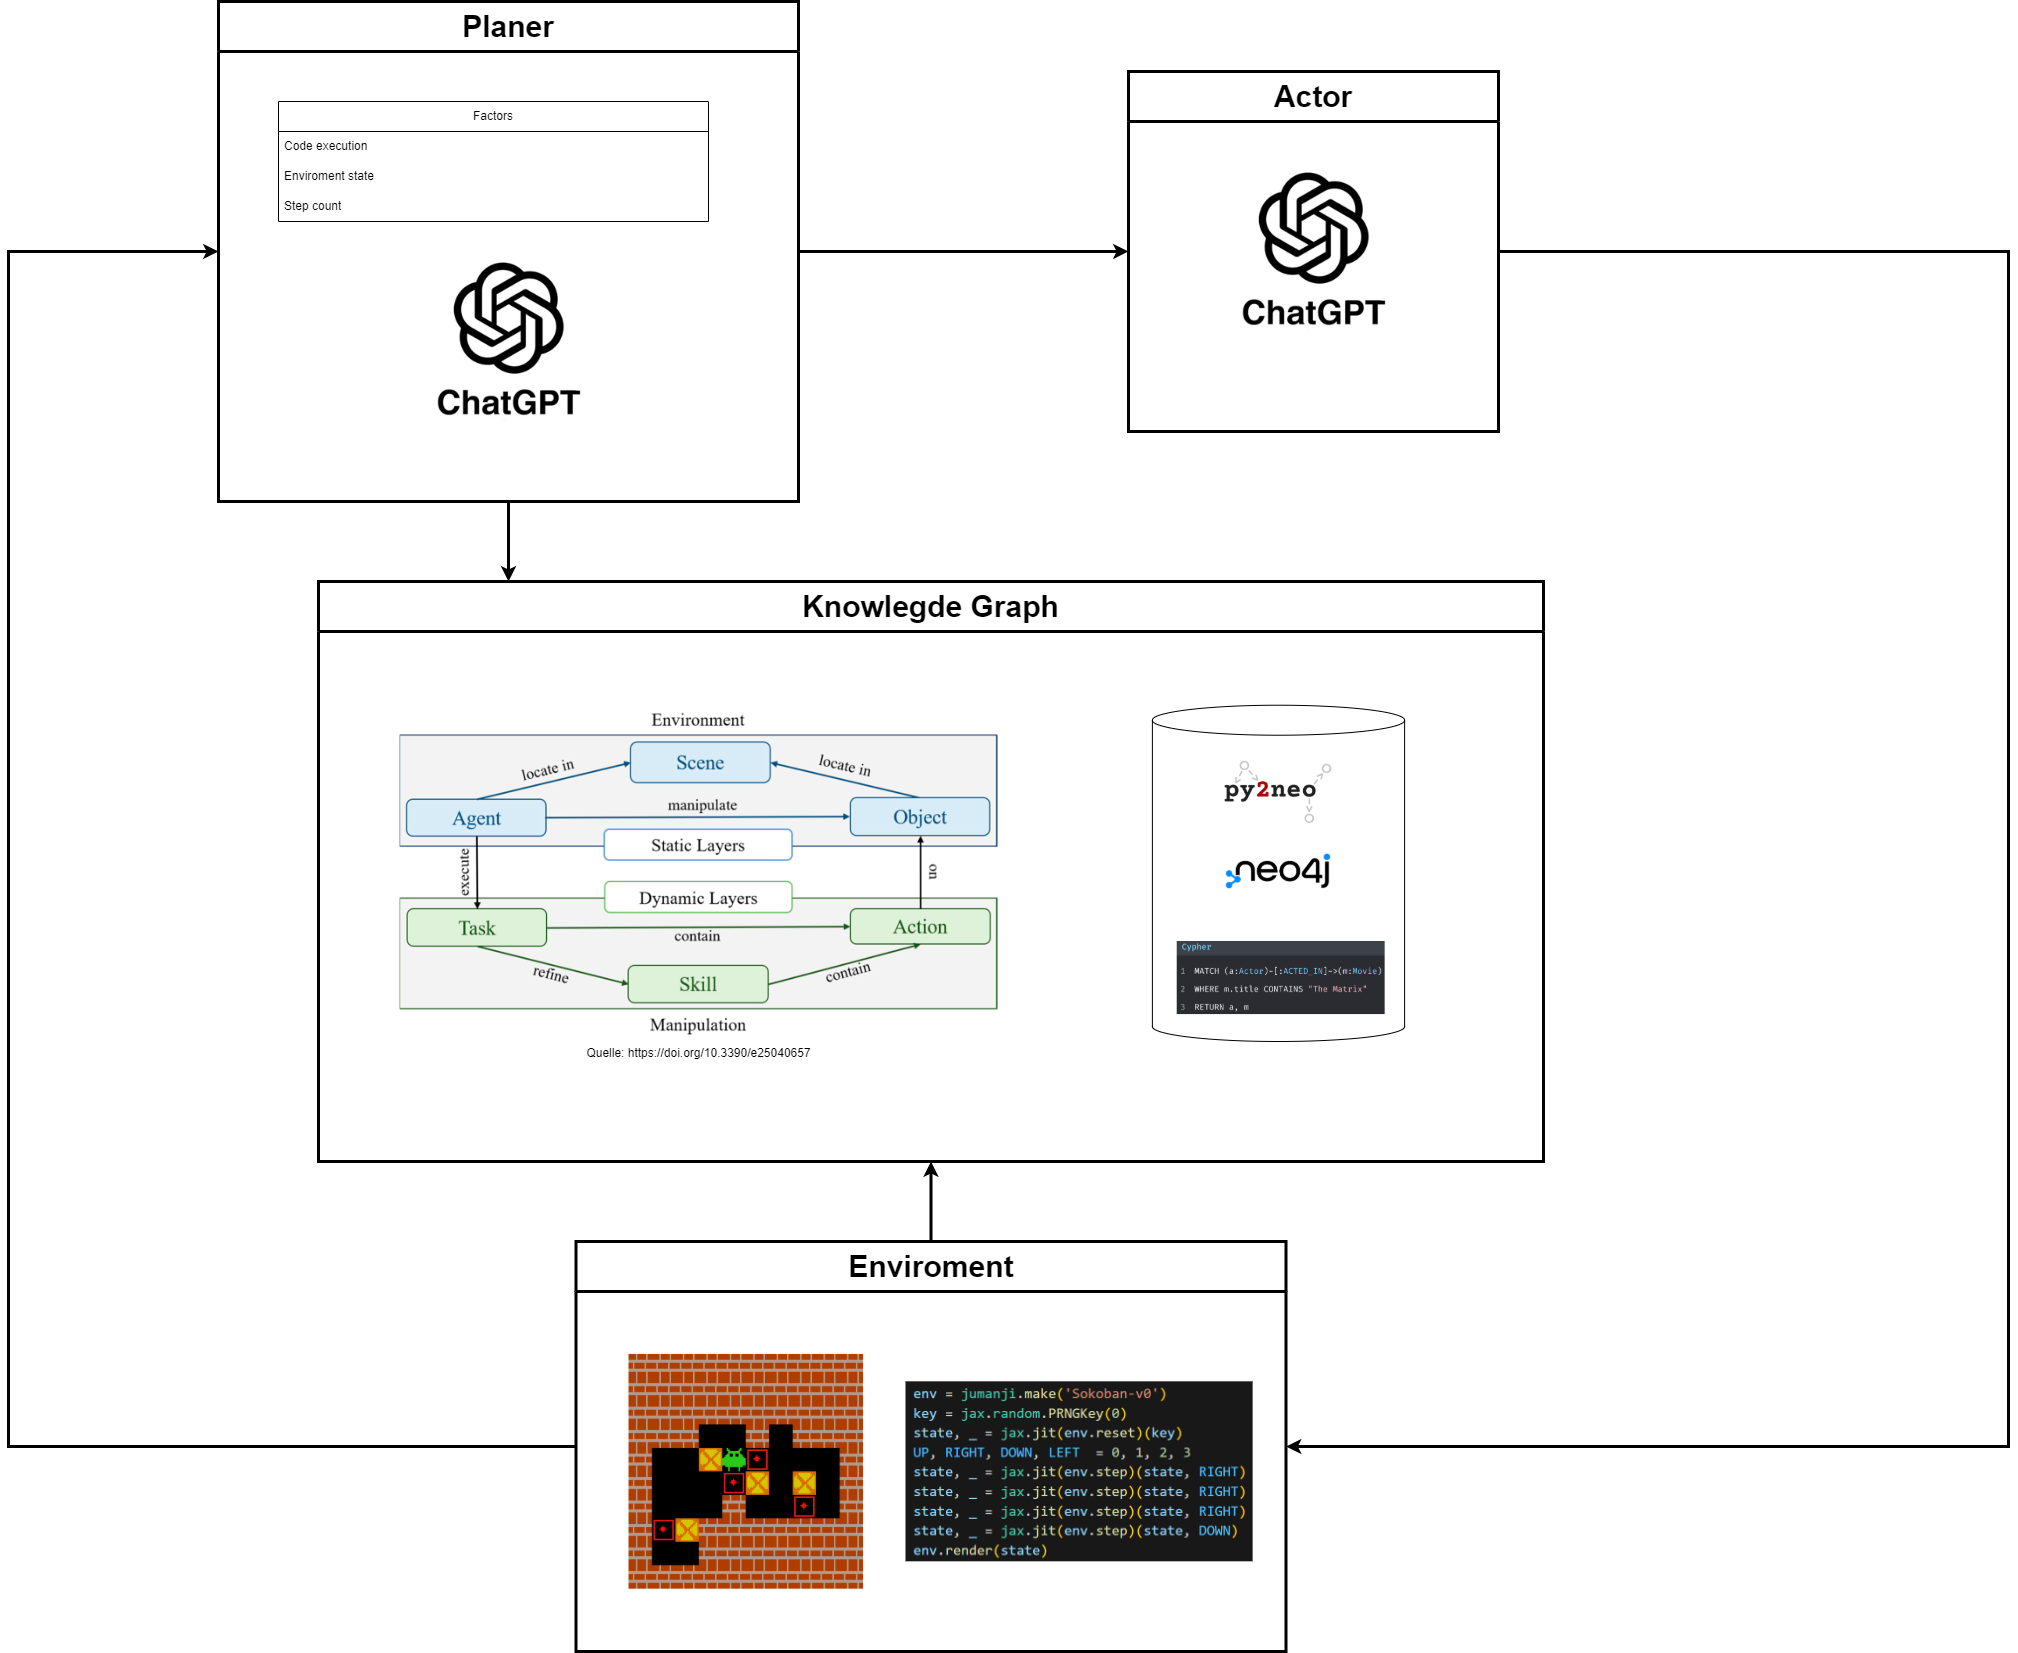
\includegraphics[height=7.0cm]{images/CodeGenKgArchitecture.png}
		\caption[Architektur]{Architektur}
	\label{Fig:CodeGenKgArchitecture}
\end{figure}

\newpage
\thispagestyle{empty}
\section*{Abstract}
\label{sec:abstract}

Englische Übersetzung der Kurzfassung (Zusammenfassung) der Arbeit auf max. 1 Seite

\tableofcontents
\newpage
\listoffigures
\newpage
\listoftables
\section*{Nomenclature}
\markright{Nomenclature}
\renewcommand{\arraystretch}{1.0}
%\begin{tabularx}{\textwidth}{l>{\raggedright}Xl}
\begin{longtable}[l]{@{}lp{12.25cm}l@{}}
	$A$               &Beschreibung                                   
\end{longtable}
\addtocounter{table}{-1}
\newpage
\pagenumbering{arabic}
\section{Einleitung}
\label{sec:Aufgabenstellung}

Einleitung auf max 1. Seite \\
- Problemstellung  \\
- Ziele der Arbeit \\
\section{Code Generation}
\label{Sec:Code Generation}



\section{Knowledge Graph}
\label{Sec:Knowledge Graph}



\section{Umgebung}
\label{Sec:Umgebung}

In diesem Abschnitt wird die Umgebung Sokoban beschrieben.~\cite{schrader_gym-sokoban_2018}

% ******************************************************************************************************************************
% Spielregel
% ******************************************************************************************************************************
\subsection{Spielregel}
\label{Subsec:Spielregel}

\begin{table}[htb!]
	\centering
	\caption[Aktionen]{Aktionen}
	\vspace{2mm}
	\begin{tabular}{c}
	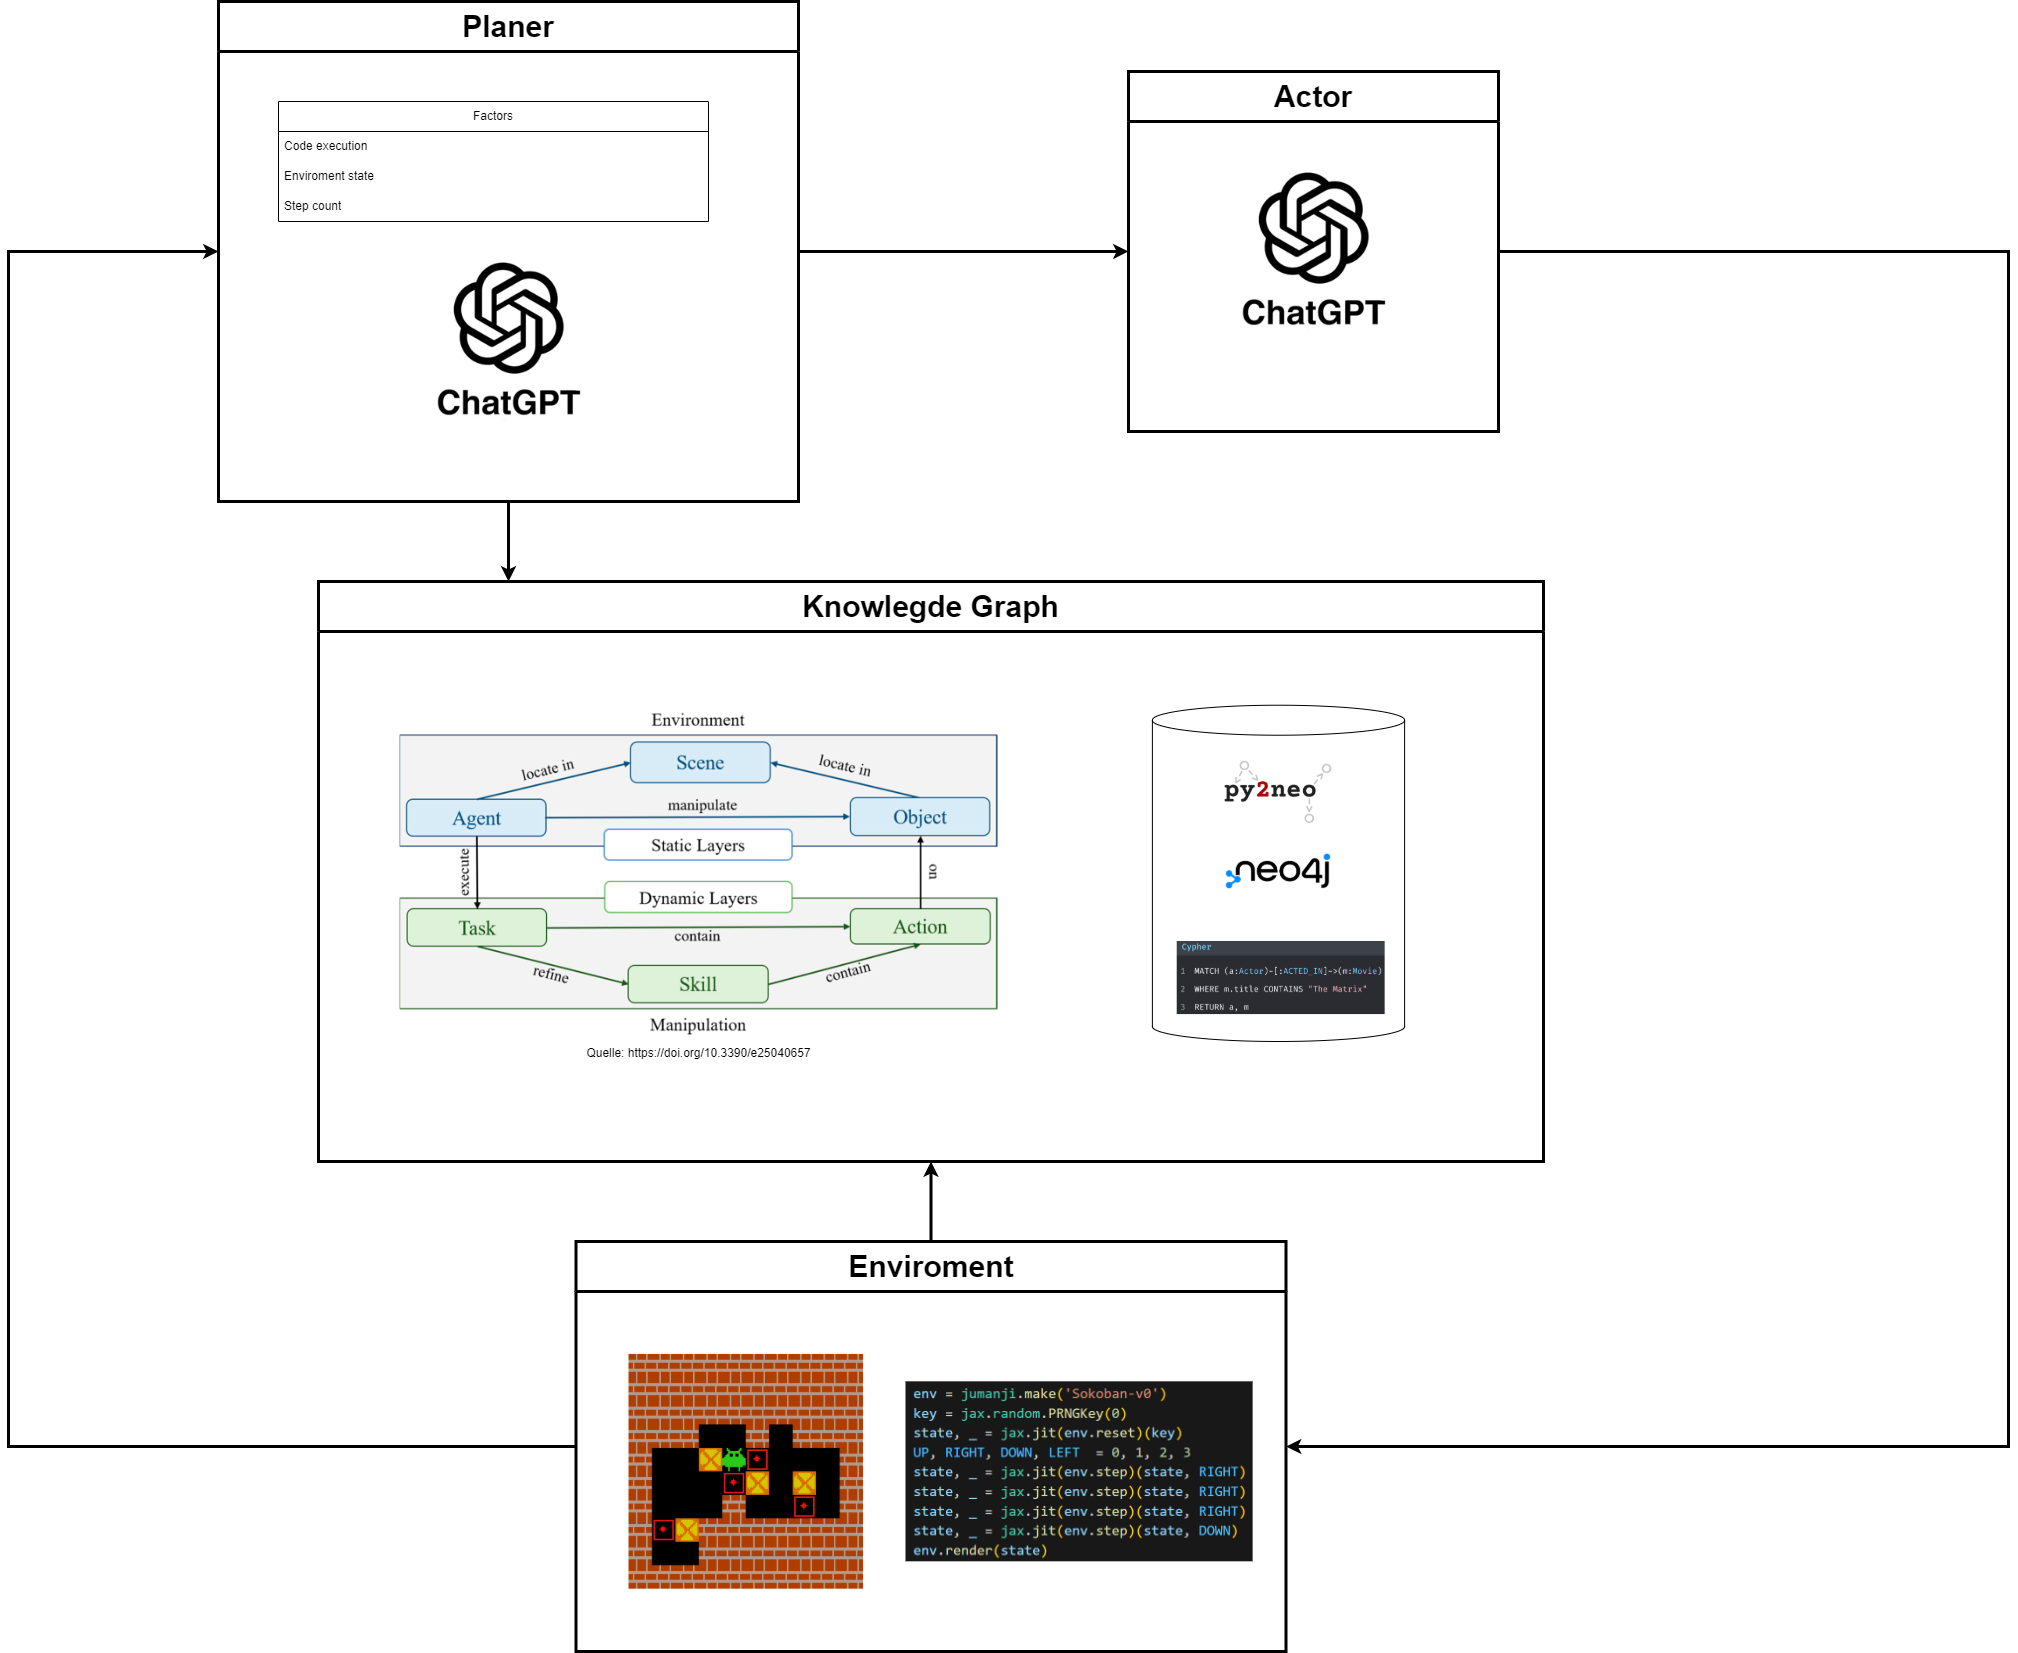
\includegraphics[width=11cm]{images/CodeGenKgArchitecture.png}
	\end{tabular}
	\label{Tab:Aktionen}	
\end{table}

% ******************************************************************************************************************************
% Besipiel
% ******************************************************************************************************************************
\subsection{Besipiel}
\label{Subsec:Besipiel}

\section{Zusammenfassung und Ausblick}
\label{Sec:Zusammenfassung_und_Ausblick}

Zusammenfassung der Arbeit und Ausblick, was noch gemacht werden muss/kann auf 1-2 Seiten.
\printbibliography[title=Literaturverzeichnis]
\thispagestyle{empty}
\section*{Eidesstattliche Erklärung}
\label{Sec:Eidesstattliche Erklärung}

Hiermit versichere ich, die vorliegende Arbeit selbstständig und nur unter Verwendung der von mir angegebenen Quellen und Hilfsmittel verfasst zu haben. Sowohl inhaltlich als auch wörtlich entnommene Inhalte wurden als solche kenntlich gemacht. Die Arbeit hat in dieser oder vergleichbarer Form noch keinem anderem Prüfungsgremium vorgelegen. \\
[1.5cm]
Datum:	\hrulefill\enspace Unterschrift: \hrulefill
\\
\begin{flushright}
Roger Näf \\[1.5cm]
\end{flushright}


% Anhang
% \appendix
% \include{chapters/91_Anhang}

\end{document}

